%%--------------------------------------------------------------------------
%%  SECTION 3: INVERSE PROBLEMS WITH DIFFUSION MODELS
%%--------------------------------------------------------------------------
\section{Learned Priors and Diffusion Models for PDE Inverse Problems}

\noindent\textit{Why it matters.}\enspace
Inverse problems in PDEs---recovering unknown fields (subsurface velocities,
source terms, initial conditions) from indirect, noise-corrupted observations---arise
throughout geophysics, medical imaging, and materials science.  Their fundamental
difficulty is \emph{ill-posedness}: the map from observations to underlying parameters
fails to be injective, so infinitely many parameter fields can explain any given data
set, and the reconstruction is acutely sensitive to noise.

Mathematically, classical approaches add a hand-crafted regularizer $\mathcal{R}(u)$
to the data-misfit objective:
\[
  \min_{u}\; \mathcal{L}_{\mathrm{data}}(u) + \lambda\,\mathcal{R}(u).
\]
Standard choices---Tikhonov, total variation, sparsity penalties---are based on
geometric intuitions (smoothness, piecewise constancy) that cannot capture the
complex statistical structure of real physical fields.  Data-driven neural networks
can learn richer priors but classically require large paired datasets of
(observation, ground-truth parameter) that are prohibitively expensive to acquire in
scientific settings.

The central thesis of our research in this area is that \emph{score-based diffusion
models} offer a principled escape from this dilemma.  Diffusion models, trained on
\emph{unpaired} samples of the unknown parameter field $u$, learn to approximate the
score $\nabla_{u}\log p(u)$ of the true prior distribution.  Because real physical
fields inhabit a low-dimensional manifold embedded in a nominally high-dimensional
parameter space, the trained score function implicitly encodes this manifold geometry.
At inference time, the learned score acts as a \textbf{data-informed regularization
signal} that guides the reconstruction toward physically plausible configurations---without
requiring a single paired training example and without embedding the forward solver in the
prior-training loop.

\begin{figure}[H]
  \centering
  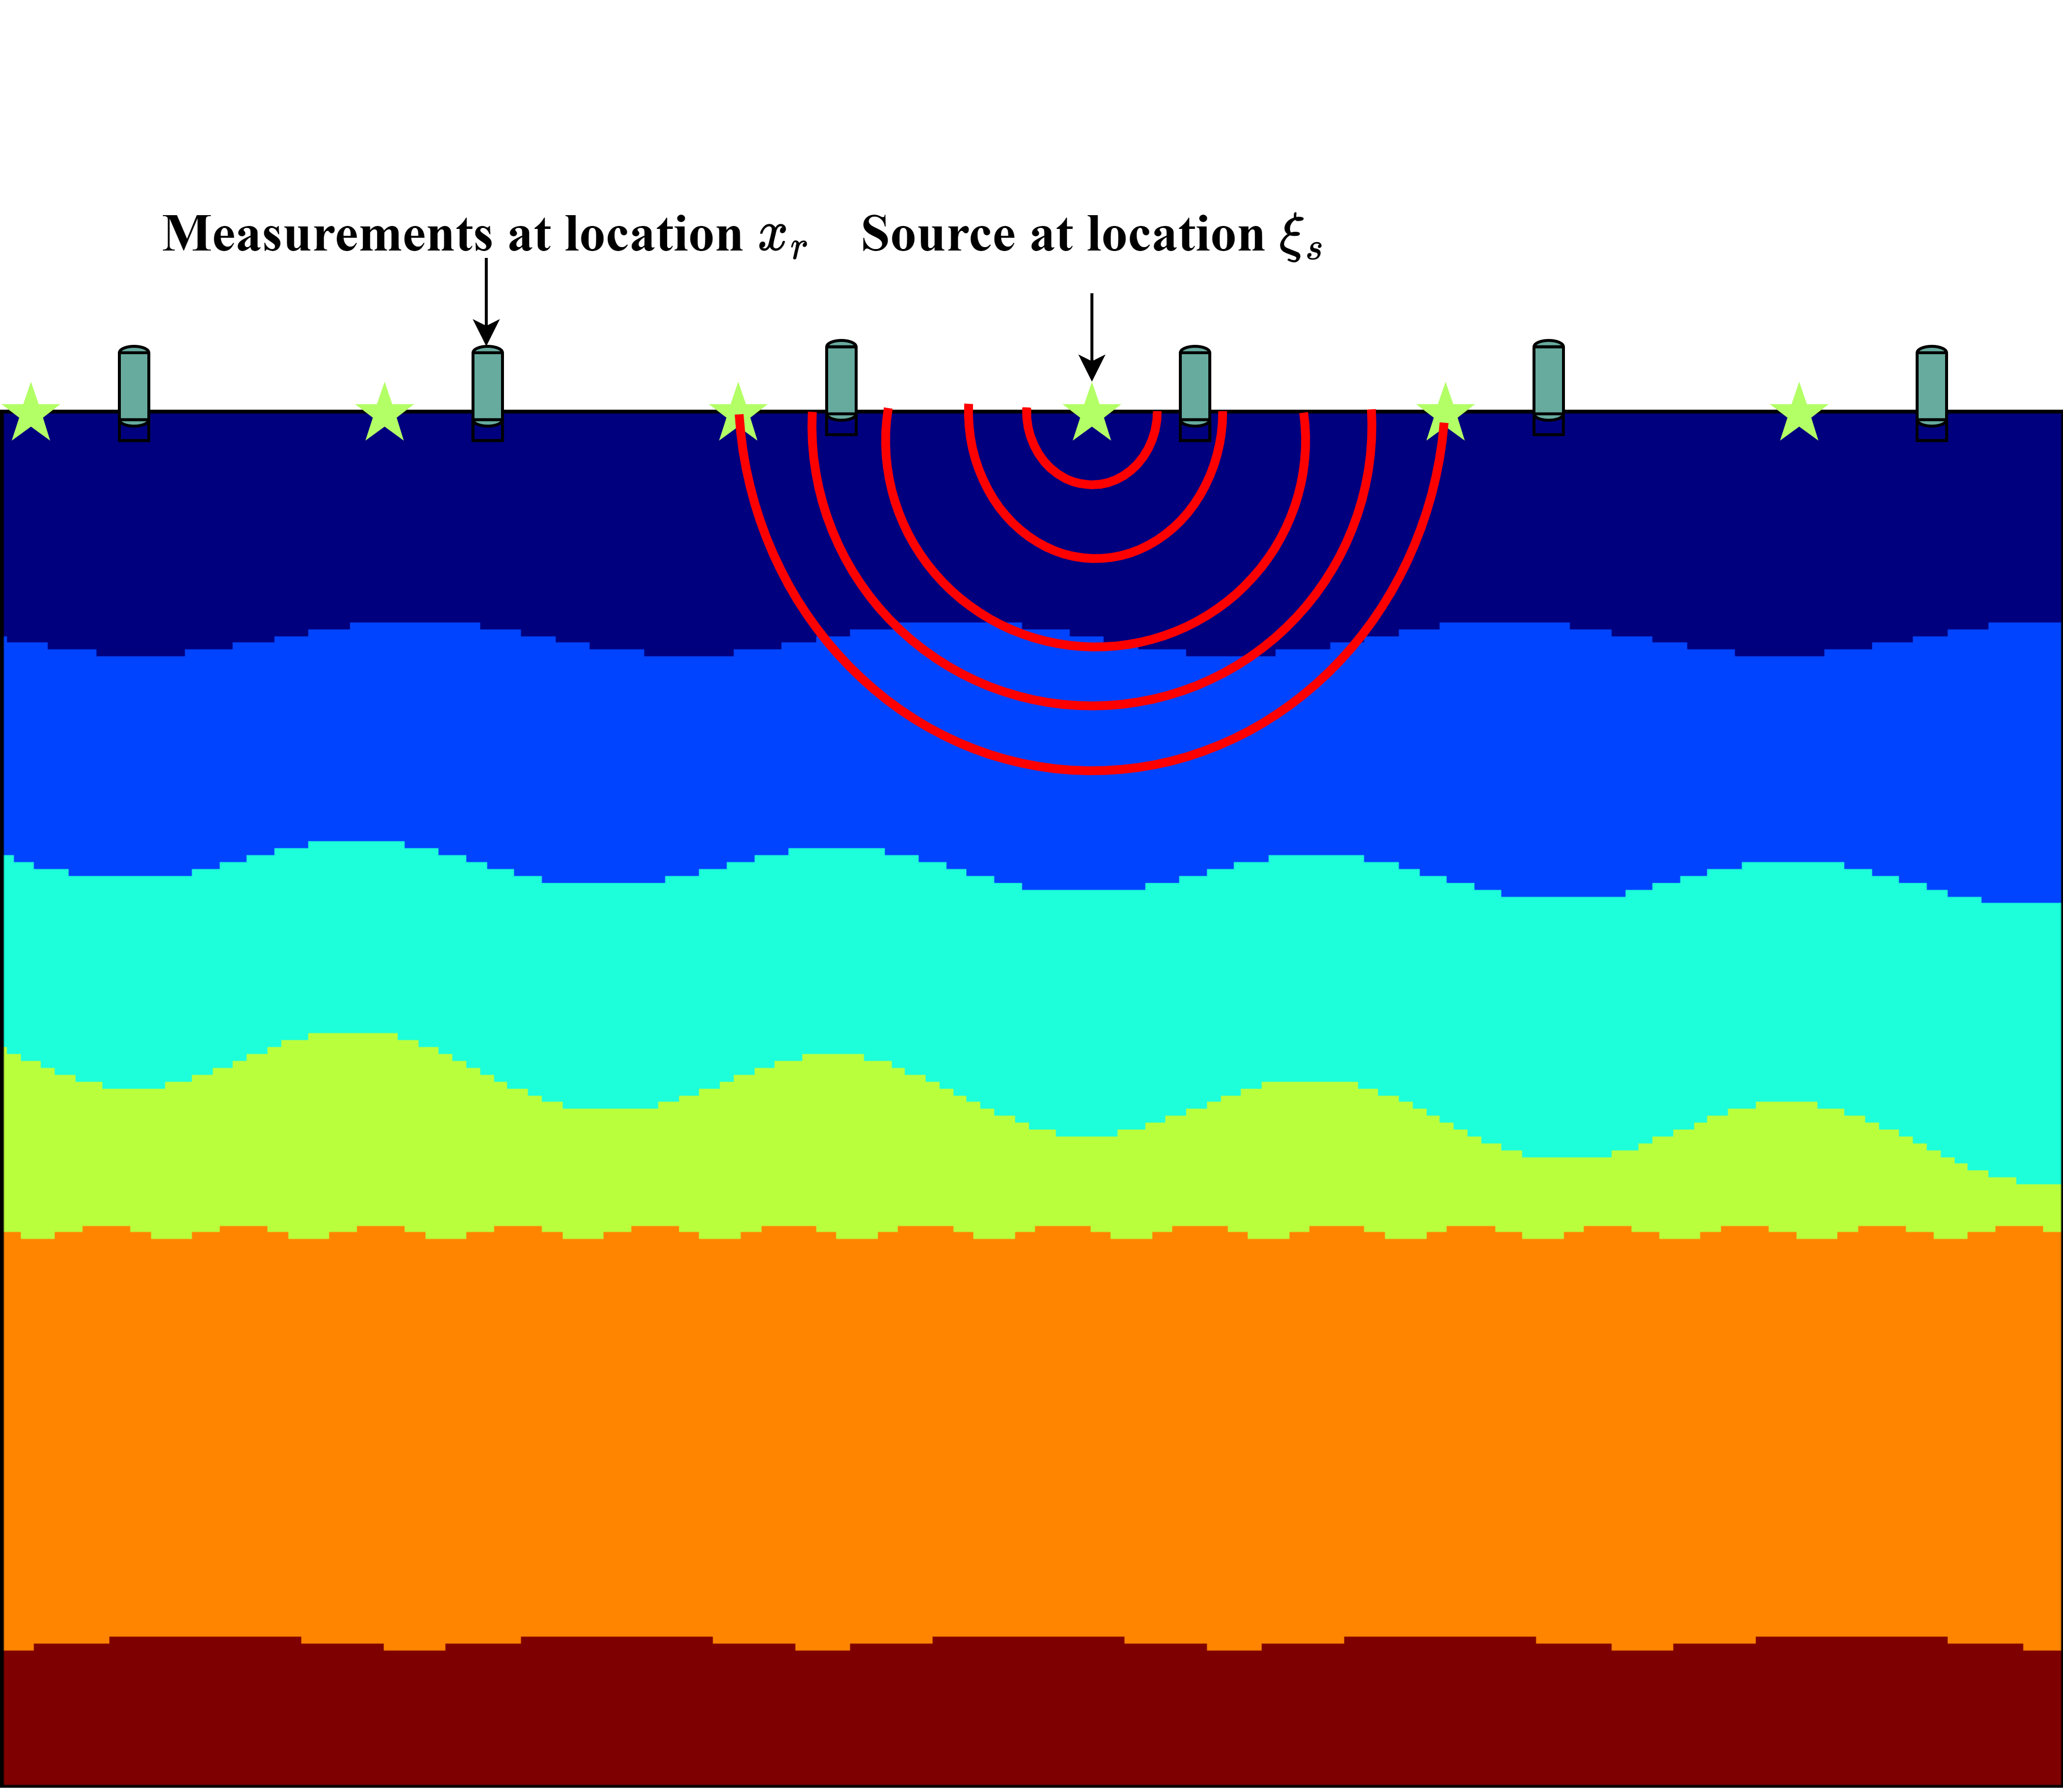
\includegraphics[width=0.45\textwidth]{figures/fwi.png}
  \caption{Illustration of the full-waveform inversion (FWI) setting: seismic
    sources (yellow stars) generate elastic waves (red arcs) that propagate through
    layered subsurface media; receivers (grey cylinders) record the resulting
    wavefields.  FWI seeks to recover the velocity structure of the subsurface
  from these surface recordings---an archetypal ill-posed PDE inverse problem.}
  \label{fig:fwi-setup}
\end{figure}

We have developed a progressive research programme applying these ideas to
PDE inverse problems, with \emph{full-waveform inversion} (FWI) as the primary
testbed.  FWI aims to recover a spatially varying wave speed $v(\mathbf{x})$ from
seismic recordings; the forward map is governed by the acoustic wave equation
\[
  \frac{1}{v^{2}(\mathbf{x})}\,\partial_{tt}u - \Delta u = s(\mathbf{x},t),
\]
and the inversion is notorious for a non-convex misfit landscape littered with
cycle-skipping local minima.  Below we summarise our three works in this line.

%- - - - - - - - - - - - - - - - - - - - - - - - - - - - - - - - - - - - - - -
\subsection{Unsupervised Bayesian Re-parametrization for Wave-Equation Inversion}

Our first work in this direction~\cite{FWI-DL2025} introduced an
\emph{unsupervised deep learning} approach to FWI that requires no paired
(seismic data, velocity model) examples whatsoever.  The key idea is a
\textbf{neural re-parametrization}: rather than optimising the velocity $v$
directly on a grid, we write $v = f_{\theta}(\mathbf{z}_{0})$, where
$\mathbf{z}_{0}$ is a \emph{fixed} random tensor and $f_{\theta}$ is a
deep neural network whose weights $\theta$ are the sole degrees of freedom.

Two structural consequences follow immediately.  First, the network architecture
acts as an \emph{implicit prior}: the set $\{f_{\theta}(\mathbf{z}_{0}) : \theta\}$
is a smooth, low-dimensional manifold of plausible velocity fields, regularising the
inversion without any explicit penalty term.  Second, by interpreting $\theta$ as a
latent variable and applying variational Bayesian inference via the
reparametrisation trick, we obtain a principled objective that quantifies
reconstruction uncertainty alongside a point estimate---a feature absent from
classical FWI.  A pretraining strategy provides a better-than-random initialisation
and substantially accelerates convergence.

Extensive numerical experiments demonstrate that this approach outperforms
conventional gradient-based FWI on challenging benchmarks featuring complex
subsurface structures and noisy measurements, establishing the viability of
implicit neural priors for PDE-constrained inversion.

\begin{figure}[H]
  \centering
  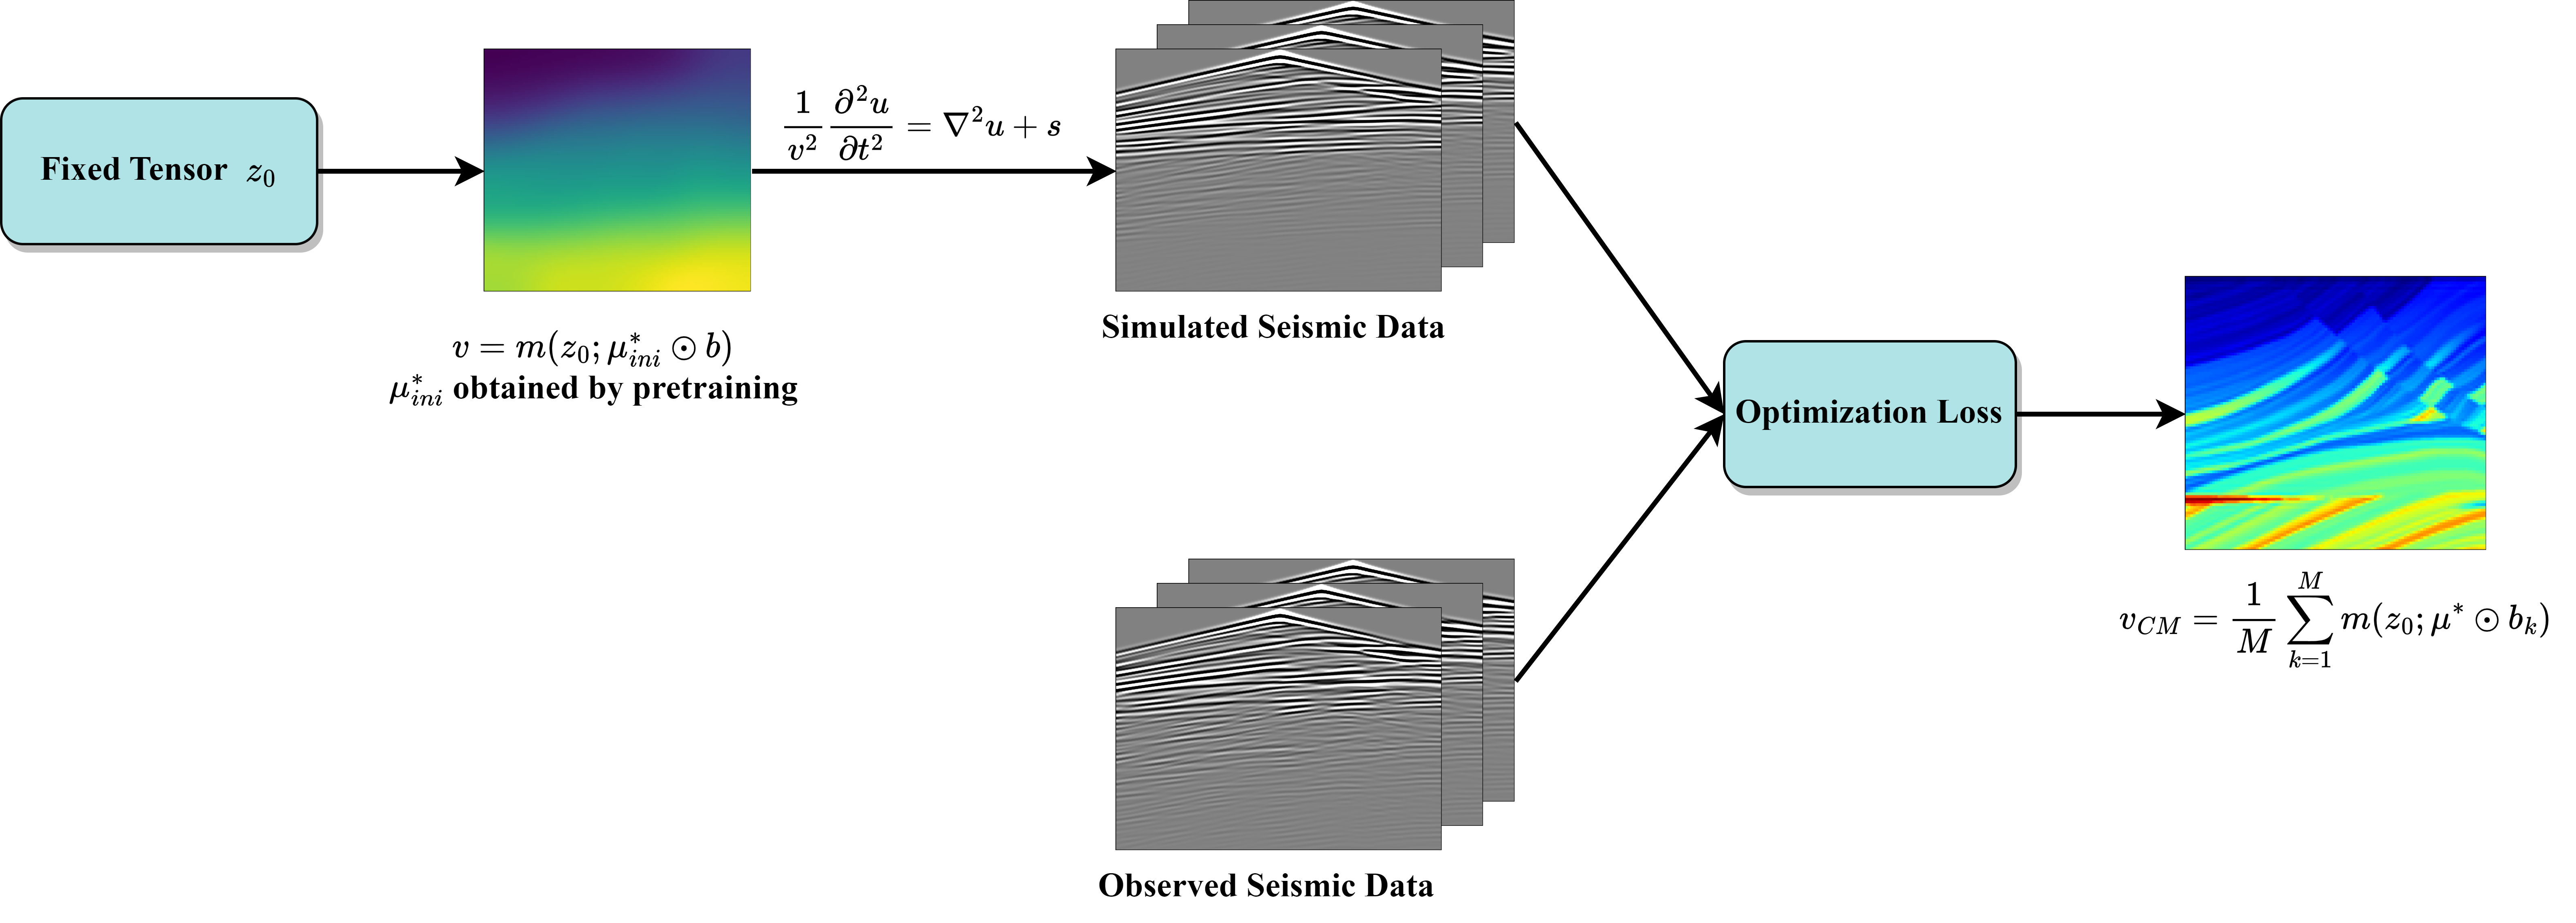
\includegraphics[width=0.8\textwidth]{figures/unsupervised_fwi.png}
  \caption{Neural re-parametrization for unsupervised FWI: a fixed random tensor
    $\mathbf{z}_{0}$ is passed through a learned neural network $f_{\theta}$ to
    produce velocity models. The network architecture acts as an implicit prior,
  constraining solutions to a smooth low-dimensional manifold of plausible fields.}
  \label{fig:unsupervised-fwi}
\end{figure}

%- - - - - - - - - - - - - - - - - - - - - - - - - - - - - - - - - - - - - - -
\subsection{ODE-DPS: Score-Based Diffusion Posterior Sampling for PDE Inverse Problems}

Building on the idea of learned priors, our second work~\cite{ODE-DPS2025} develops
\textbf{ODE-DPS}\@, a fully diffusion-based framework for solving inverse problems
across a general class of PDEs.  The approach casts PDE inversion as \emph{Bayesian
posterior sampling}: given noisy observations $y^{\delta} = \mathcal{F}(\bar{u}) + \xi$,
the posterior $p(\bar{u}\,|\,y^{\delta})$ concentrates on physically consistent
solutions.  A score-based diffusion model trained on samples of $\bar{u}$ (no pairing
with observations required) supplies the prior score
$\nabla_{\mathbf{x}}\log p_{0}(\mathbf{x})$, while posterior sampling proceeds by
reversing the noising dynamics,
\[
  d\mathbf{x} = \!\left[-\tfrac{\beta(t)}{2}\mathbf{x} - \beta(t)\,
  \nabla_{\mathbf{x}}\log p(\mathbf{x}(t))\right]dt
  + \sqrt{\beta(t)}\,d\bar{\omega},
\]
with a likelihood-guidance correction injected at each step.

\begin{figure}[H]
  \centering
  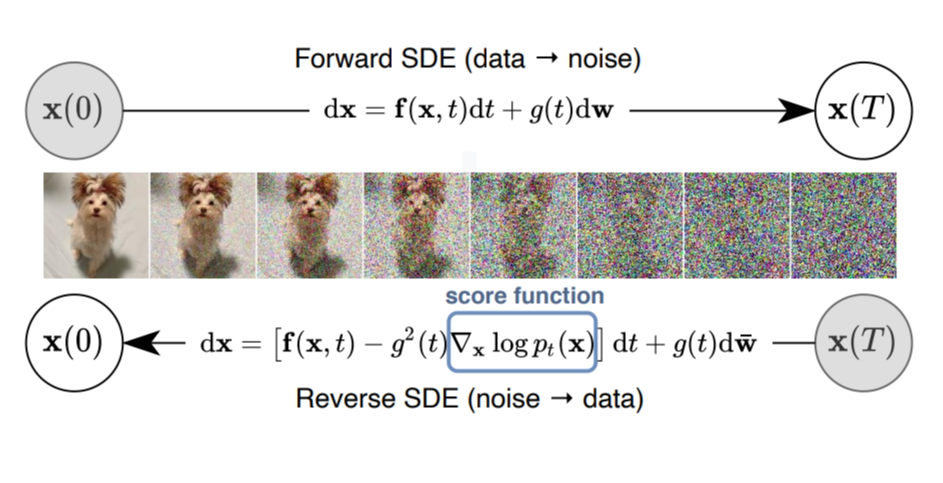
\includegraphics[width=0.6\textwidth]{figures/dm.png}
  \caption{Illustration of score-based diffusion models: a learned score function
    $\nabla_{\mathbf{x}}\log p(\mathbf{x}(t))$ guides the reverse noising process
  from pure noise toward samples of the true prior distribution.}
  \label{fig:diffusion-model}
\end{figure}

The critical algorithmic contribution is an \textbf{ODE-based variant} that replaces the
stochastic reverse dynamics with a deterministic probability-flow ODE.  The key
observation is that two distinct forward noising processes can yield marginals satisfying
the same Fokker--Planck equation; their corresponding reverse ODEs therefore converge to
identical data distributions.  Exploiting this equivalence produces a \emph{more stable
and accurate} inversion trajectory than the standard SDE sampler.  An additional adaptive
norm modification---replacing the $\ell_{2}$ data-residual term with a spatially weighted
norm---reduces reconstruction errors near domain boundaries.  The method is validated
across multiple PDE inverse problems (heat source recovery, wave-equation inversion),
consistently outperforming classical Tikhonov and Landweber iteration baselines.

%- - - - - - - - - - - - - - - - - - - - - - - - - - - - - - - - - - - - - - -
\subsection{Robust Physics-Guided Diffusion for Full-Waveform Inversion}

The most recent and technically advanced work in this line~\cite{Peng2026} targets
the specific challenges of FWI: \emph{phase/amplitude imbalance} in seismic traces,
\emph{cycle-skipping} in the gradient landscape, and the need for stable guidance
throughout a long reverse-diffusion trajectory.  We present a \textbf{robust
physics-guided diffusion} framework with two principal innovations.

\textbf{Wasserstein-2 data-consistency potential.}  Standard DPS uses a pointwise
$\ell_{2}$ misfit between observed and synthetic seismograms, which is devastatingly
sensitive to phase shifts and amplitude imbalance.  We replace it with a
one-dimensional Wasserstein-2 (optimal-transport) objective computed per
source--receiver trace.  Treating each trace as a probability density, the $W_2$
distance compares quantile functions, making the guidance signal
invariant to common seismic artefacts and alleviating cycle-skipping.

\textbf{Preconditioned guided reverse-diffusion.}  The uniform scalar step size in
standard DPS is poorly matched to the spatially heterogeneous geometry of velocity
models.  We replace it with a \emph{diagonal preconditioner} $P_{i} = \rho_{i}D_{i}$
that adapts the guidance strength and spatial scaling across both diffusion steps and
spatial locations.  A conservative guidance schedule in early reverse-time steps (when
the denoised estimate is still rough) and increasingly aggressive guidance as the
estimate sharpens further stabilise the trajectory.

Numerical experiments on the full suite of OpenFWI benchmarks (CurveVel-A/B,
FlatFault-A/B, CurveFault-A/B) demonstrate that our method attains the lowest
reconstruction error and highest image-quality metrics (PSNR, SSIM) among all
competing methods---including deterministic optimisation baselines and the original
DPS---under matched computational budgets (Table.~2 in~\cite{Peng2026}). The
improvement is especially pronounced on the most challenging CurveFault benchmarks,
where the combination of curved interfaces and sharp fault discontinuities stresses
both classical and standard diffusion-based inversions.

\bigskip
\noindent\textbf{Outlook.}  This research programme establishes a cohesive vision:
by learning a low-dimensional manifold prior from unpaired physical field samples,
score-based diffusion provides a rigorous, data-informed alternative to hand-crafted
regularisers for any ill-posed PDE inverse problem.  Open directions include extension
to 3-D seismic domains, multi-physics inversion (elastic or viscoelastic wave
equations), and theoretical analysis of the posterior concentration rate as a function
of data quality and model expressivity.
